\scanpage{116}

\[ X\lhook\joinrel\relbar Y \]

\[ X_0\ X_1\ \cdots \]

\deleted{$X\lhook\joinrel\relbar Y$}

\[ \unsure{\mathbb Q|Q}_\ell \]

\diagram{\begin{tikzcd}[ampersand replacement=\&] X_0\arrow[r,hook,no head,"i"'] \& X\arrow[r,hook,no head,"f"'] \& Y \end{tikzcd}}

$X$ \uline{régulier}

\figure{
\begin{tikzpicture}[scale=.42]\draw (0,3.5) .. controls (0,2.8) and (-.15,2.3) .. (.5,1.85); \draw (.45,3.25) .. controls (.03,2.3) and (-.03,1.4) .. (-.02,0); \draw (0,1.35) .. controls (.03,1.02) and (.25,.88) .. (.53,.66); \draw (.38,1.61) .. controls (-.03,1.1) and (-.10,.35) .. (-.02,0);\end{tikzpicture}}

\[ i_!(\mathbb Q_{\ell X_0})\longrightarrow {}^{\unsure{\uparrow|t}}R i_*(\mathbb Q_{\ell X_0}) \]

\unsure{4|$\hookleftarrow$}

\textcircled{1} $X$ \uline{régulier}, $F=\mathbb Q_{\ell X}$, $f$ immersion \quad $(n=\dim\overline{f(x)})$

On peut supposer $X\longrightarrow Y$ imm. \uline{ouverte}

\diagram{\begin{tikzcd}[ampersand replacement=\&,column sep=small,row sep=small] {} \& Y'\arrow[d,"h"] \\ X\arrow[ur,hook,no head,"g"]\arrow[r,hook,no head,"f"'] \& Y \end{tikzcd}}

$Y'$ régulier, $Y'-g(X)=\deleted{\unsure{Z}}h^{-1}(Y-X)=Z$ diviseur à crois$^{\rm mt}$ norm$^{\rm x}$ \quad $Z=\sum Z_i$

\[ \deleted{\unsure{H}}\ R^*f_*(\mathbb Q_{\ell X})\Leftarrow E_2^{pq}=R^p h_*(R^qg_*(\mathbb Q_\ell)\unsure{(-1)))} \]

\[ R^qg_*(\mathbb Q_\ell)=\bigwedge^{q}\sum\mathbb Q_{\ell Z_i}=\sum_{i_1<\cdots<i_q}\mathbb Q_{\ell Z_{i_1}\cap\cdots\cap Z_{i_q}}(-q \]

\margin{$X\lhook\joinrel\relbar$}

pur de poids $2q$

\[
\begin{aligned}
E_2^{p0}=R^p h_*(\mathbb Q_{\ell\deleted{\unsure{X_0}}Y'})&\quad\text{est eff$^{\rm t}$ admissible de poids }\leq p=i\\
&\quad\text{niveau }\leq\operatorname{Inf}(p,2n-2-p\\
&\quad[\text{\unsure{au complet si|au compl. si|avec égalité si}}\ \deleted{\unsure{\leq 4p}}\ p\geq n-1]
\end{aligned}
\]

\[
\begin{aligned}
E_2^{pq}=\sum_{i_1<\cdots<i_q} R^p f_{Z_{i_1}\cap\cdots\cap Z_{i_q}*}(\mathbb Q_\ell)(-q)&\quad\text{est eff. admissible}\\
&\text{de poids }\leq p+2q=i+q\ \deleted{\leq}\leq 2n\deleted{\unsure{-2}}\\
&\text{de niveau }\leq\operatorname{Inf}(p,2n-2q-p)
\end{aligned}
\]

\[ p\deleted{\unsure{\leq}}\ 2(n\deleted{\unsure{q}}-q)\,/\,p \]

\[ \text{\textcircled{\unsure{Pds|5.e}}}\quad i+q=\boxed{\begin{aligned}p+2q&\leq 2n\deleted{\unsure{-2}}\\ q&\leq n,2n-i\end{aligned}} \]

\[
\begin{aligned}
&\text{en tous cas, poids entre }\ \text{\tikz[baseline=(a.base)]\node[draw,ellipse,inner sep=2pt](a){$\leq\deleted{\unsure{2i}}$};}\operatorname{Inf}(2i,2n-2\\
&\text{niveau }\leq\deleted{\unsure{2i-p}}\operatorname{Inf}(i,2n-2-i)
\end{aligned}
\]

\figure{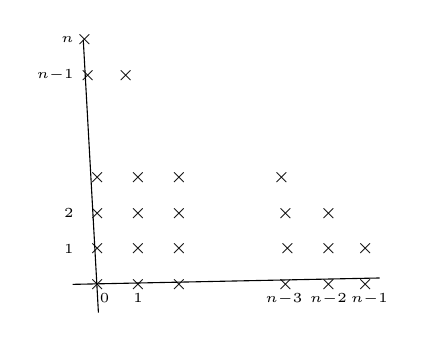
\begin{tikzpicture}[x=.52cm,y=.45cm]
\draw (-.6,0)--(6.9,.18); \draw (.03,-.8)--(-.34,6.9);
\foreach \x/\y in {0/0,1/0,2/0,4.6/0,5.65/0,6.55/0,0/1,1/1,2/1,4.65/1,5.65/1,6.55/1,0/2,1/2,2/2,4.6/2,5.65/2,0/3,1/3,2/3,4.5/3,-.23/5.9,.70/5.9,-.31/6.9}{\node[inner sep=0pt] at (\x,\y) {$\scriptstyle\times$};}
\foreach \x/\lab in {.18/0,1/1,4.56/{n-3},5.65/{n-2},6.65/{n-1}}{\node[below] at (\x,.02) {$\scriptscriptstyle\lab$};}
\foreach \y/\lab in {1/1,2/2,5.9/{n-1},6.9/n}{\node[left] at (-.34,\y) {$\scriptscriptstyle\lab$};}
\end{tikzpicture}}

\[ \begin{aligned}p&\leq n-1\\q&\leq n\end{aligned} \]

\[ \begin{aligned} &p\qquad \unsure{n+q|n-q}\\[-2pt] &\overbrace{p+q\geq n}\end{aligned} \]

\[ \begin{aligned}2(p-n+q)&=2(i-n)\qquad \unsure{2n-2}-\\ 2(n-q)-p&=\underline{2n-i}-q\end{aligned}\qquad 2. \]

% archive sheet number: 115
